\section{Double Side-Band with Carrier}
The second option for transmitting a carrier along with the modulated signal is
the choice in broadcasting because of its desirable trade-offs. This leads to so called (amplitude modulation), in which the transmitted signal is given by,

\begin{equation}
	\begin{split}
	\varphi_{AM} & =A\cos{\omega_ct}+m(t)\cos{\omega_ct} \\
	 & =[A+m(t)]\cos{\omega_ct} 
	\end{split}
\end{equation}

The spectrum $\phi_{AM}(t)$ is basically the same as that of $\varphi_{DSB-SC}(t)=m(t)\cos{\omega_ct}$ except for the two
additional impulses at $\pm f_c$ .
\begin{equation}
	\varphi_{AM}(t) \Leftrightarrow \frac{1}{2}[M(f+f_c)]+\frac{A}{2}[\delta(f+f_c)+\delta(f-f_c)]
\end{equation}

If A is not sufficient amount for which $m(t)+A$ is always $\geq 0$ then, envelope detection will not work.

\begin{figure}[H]
	\centering
	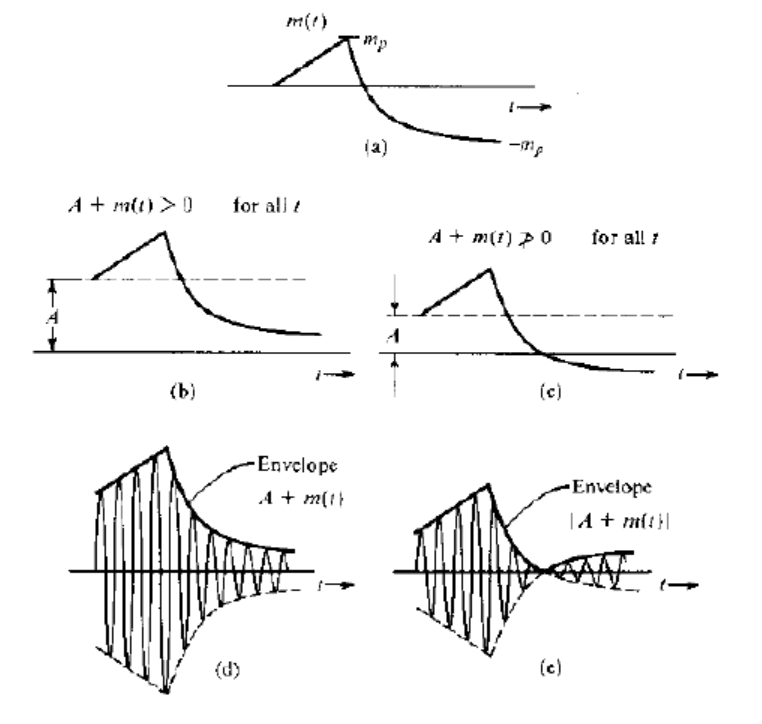
\includegraphics[]{Capture4.PNG}
\end{figure}

\begin{figure}[H]
	\centering
	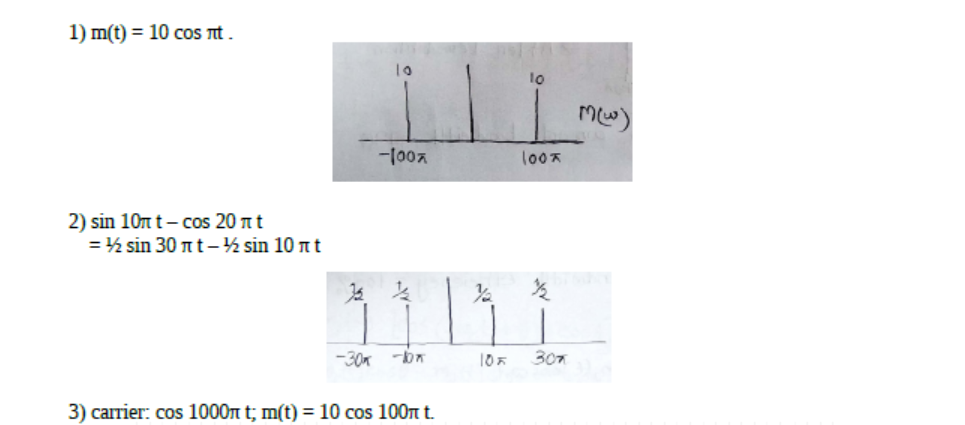
\includegraphics[]{Capture5.PNG}
\end{figure}

\begin{figure}[H]
	\centering
	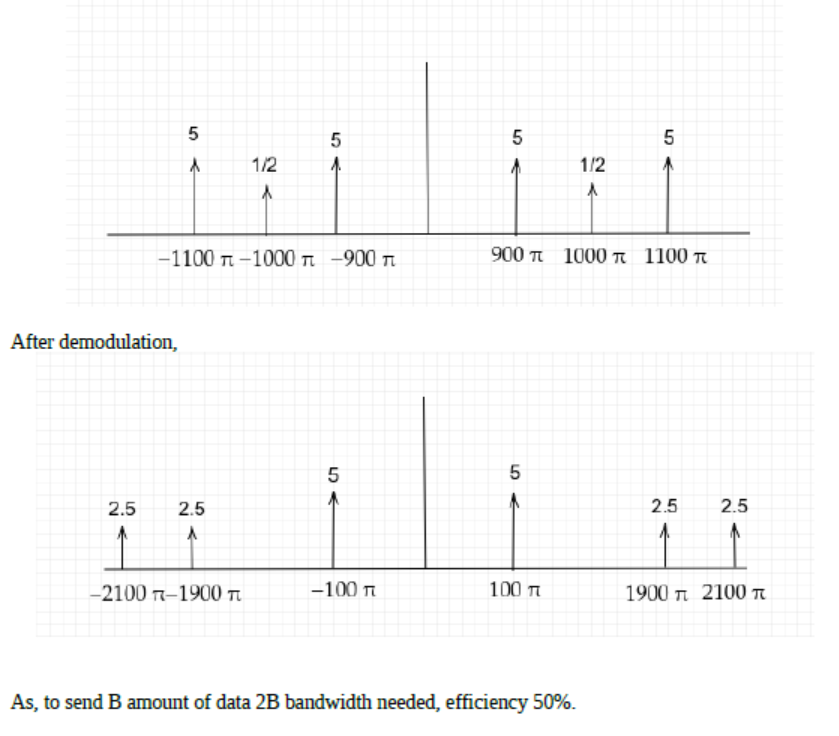
\includegraphics[]{Capture6.PNG}
\end{figure}


\section{Quadrature Amplitude Modulation}

\begin{figure}[H]
	\centering
	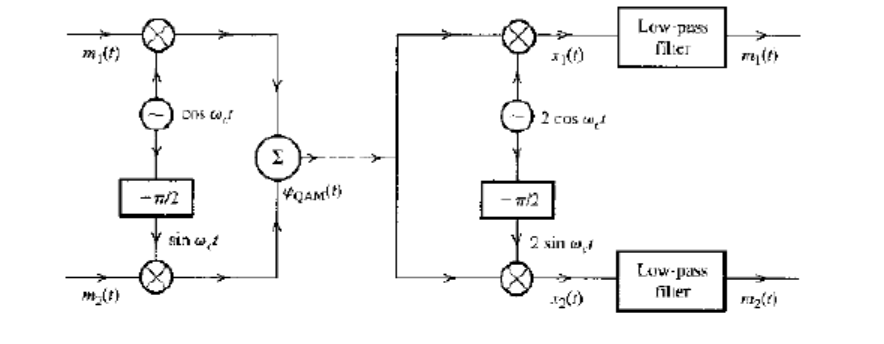
\includegraphics[]{Capture7.PNG}
\end{figure}

Modulation:

\begin{equation}
	\varPhi_{QAM}(t)=m_1(t)\cos{\omega_ct}+m_2(t)\sin{\omega_ct}
\end{equation}

Demodulation:

\begin{equation}
	\begin{split}
	x_1(t) & =2\varPhi_{QAM}(t)\cos{\omega_ct}\\
	& = 2[m_1(t)\cos{\omega_ct}+m_2(t)\sin{\omega_ct}]\cos{\omega_ct}\\
	& = m_1(t)+ m_1(t)\cos{2\omega_ct}+m_2(t) \sin{2\omega_ct}
	\end{split}
\end{equation}

\begin{equation}
	\begin{split}
	x_2(t) & =2\varPhi_{QAM}(t)\sin{\omega_ct}\\
	& = 2[m_1(t)\cos{\omega_ct}+m_2(t)\sin{\omega_ct}]\sin{\omega_ct}\\
	& = m_2(t)- m_2(t)\cos{2\omega_ct}+m_1(t) \sin{2\omega_ct}
	\end{split}
\end{equation}

Thus, two baseband signals, each of bandwidth B Hz, can be transmitted simultaneously over a bandwidth 2B by using DSB transmission and quadrature multiplexing.

Problem: However, QAM demodulation must be synchronous, An error in the phase or the
frequency of the carrier at the demodulation in QAM will result in loss and interference between the two channels. To show this, let the carrier at the demodulator be $2\cos{(\omega_ct+\theta)}$.

In this case,

\begin{equation}
\begin{split}
x_1(t) & = 2[m_1(t)\cos{\omega_ct}+m_2(t)\sin{\omega_ct}]\cos{\omega_ct}\\
& = m_1(t)+ m_1(t)\cos{2\omega_ct}+m_2(t) \sin{2\omega_ct}
\end{split}
\end{equation}

The low pass filter suppresses the two signals modulated by carrier of angular frequency $2\omega_c$ , resulting in the first demodulator output,

\begin{equation}
	m_1(t)\cos{\theta}-m_2(t)\sin{\theta}
\end{equation}

Thus, in addition to the desired signal $m_1(t)$, we also received signal $m_2(t)$ in the upper reciever branch.



